\documentclass[12pt]{article}
\usepackage[utf8]{inputenc}
\usepackage[T1]{fontenc}
\usepackage{fontspec}
\setmainfont{Times New Roman}
\newfontfamily\hackfont{Hack}
\usepackage{titlesec}
\usepackage{fancyhdr}
\usepackage{listings}
\usepackage{xcolor}
\usepackage{graphicx}
\usepackage{longtable}
\usepackage{caption}
\usepackage{hyperref}
\usepackage{setspace}
\usepackage{geometry}
\geometry{a4paper, margin=1in}
\hypersetup{colorlinks=true, linkcolor=blue, urlcolor=blue}
\renewcommand{\contentsname}{Table of Contents}

\pagestyle{fancy}
\fancyhf{} 							% Header Middle
\rhead{VLSI Design Lab}
\lhead{Lab-02: Sequential Circuit}
\rfoot{\thepage}

\begin{document}

\begin{titlepage}					% Cover Start
\begin{center}
    
\includegraphics[width=0.35\textwidth]{logo.png} \\
    \vspace{0.5cm}
    \textbf{\Huge \textcolor{cyan}{NOTRE DAME} \textcolor{cyan}{UNIVERSITY}} \\
    \vspace{0.5cm}
    \textbf{\Huge \textcolor{orange}{BANGLADESH}} \\
    
    \vspace{0.9cm}
    \textbf{\Huge \underline{VLSI Design Lab Report-02}} \\
    
    \vspace{1.5em}
    \begin{flushleft}
    	\textbf{\Large Course Code: CSE-4218} \\
		\vspace{0.3cm}        
        \textbf{\Large Course Title: VLSI Design Lab} \\
        \vspace{0.3cm}
        \textbf{\Large Experiment Name: Implementing Sequential Circuit} \\        
    \end{flushleft}
    
    \vspace{1em}
    \begin{flushleft}
        \textbf{\Huge \textcolor{blue}{Submitted by:}} \\
        \vspace{0.3cm}
        \textbf{\Large Name: Istiak Alam} \\
        \vspace{0.3cm}
        \textbf{\Large ID: 0692230005101005} \\
		\vspace{0.3cm}        
        \textbf{\Large Batch: CSE-20} \\
        \vspace{0.5cm}
        \textbf{\Large Submission Date: }{\Large \textbf{\today}\par}
    \end{flushleft}
    \vfill
    \begin{flushleft}
        \textbf{\Huge \textcolor{blue}{Submitted to:}} \\
        \vspace{0.3cm}
        \textbf{\Large Nfisa Tabassum,} \\
        \vspace{0.3cm}
        \textbf{\Large Lecturer, Dept. of CSE} \\
        \vspace{0.3cm}
        \textbf{\Large Notre Dame University Bangladesh}
    \end{flushleft}
\end{center}
\end{titlepage}						% Cover End

\tableofcontents
\thispagestyle{empty}
\clearpage
\pagenumbering{arabic}

\section{Introduction}
The objective of this laboratory experiment is to implement given Boolean expressions using CMOS logic and verify their functional correctness through schematic design and timing simulation. The circuits were designed using the DSCH2 schematic editor, following standard CMOS pull-up and pull-down network principles. Truth tables and timing diagrams were analyzed to validate logical behavior.


\section{Function 1: $(ABC + D)'$}

\subsection*{Boolean Function}
\[
Y = (ABC + D)'
\]

\subsection*{Truth Table}
\begin{center}
\begin{tabular}{cccc|c}
\hline
A & B & C & D & Y \\ \hline
0 & 0 & 0 & 0 & 1 \\
0 & 0 & 1 & 0 & 1 \\
0 & 1 & 0 & 0 & 1 \\
0 & 1 & 1 & 0 & 1 \\
1 & 1 & 1 & 0 & 0 \\
X & X & X & 1 & 0 \\ \hline
\end{tabular}
\end{center}

\subsection*{Schematic Image}
\begin{figure}[!h]
\centering
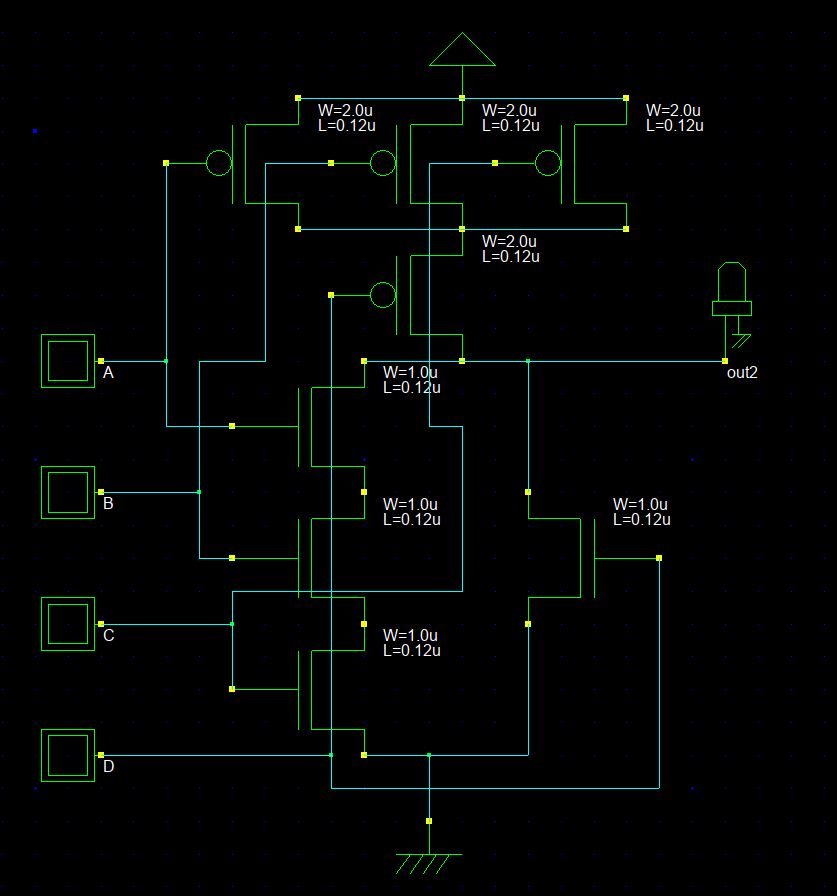
\includegraphics[width=0.7\textwidth]{output-1.png}
\caption{CMOS Schematic of $(ABC + D)'$}
\end{figure}





\section{Conclusion}
All CMOS circuits were successfully implemented and verified using DSCH2. Truth tables and timing diagrams matched theoretical expectations, confirming correct logical and temporal behavior of each function.


\end{document}